% !TeX program = lualatex

% Dokumenteneinstellungen und Infos importieren
% -------------------------------------------------------
% Informationen und Einstellungen für Ihre Abschlussarbeit
%

% Sprache für das Dokument festlegen
\newcommand{\hsmasprache}{de} %de für Deutsch oder en für Englisch


% Abgabeform festlegen
% Bei einer digitalen Abgabe, wird das Dokument einseitig erzeugt und der Titel wird
% zentriert.
\newcommand{\hsmaabgabe}{digital} % Abgabe erfolgt für Fakultät I digital. Optionen hier sind für anderen Fakultäten: "papier" oder "digital".


% Flags für Veröffentlichung, Sperrvermerk und Genderhinweis
\newcommand{\hsmapublizieren}{publizieren}   % Wird einer Veröffentlichung zugestimmt? ja=publizieren, nein=geschlossen

\newcommand{\hsmasperrvermerk}{oeffentlich} % Hat die Arbeit einen Sperrvermerk? ja=vertraulich, nein=oeffentlich, Standard ist: oeffentlich


\newcommand{\genderhinweis}{gender}     % Soll der Gender-Hinweis angezeigt werden? ja=gender, nein = nogender; Genderhinweis wird nur in deutscher Sprache angezeigt!


\newcommand{\hsmaquellcode}{sourcecode} % Verwenden Sie Quellcode in Ihrer Arbeit? ja=sourcecode, nein= nosourcecode

\newcommand{\hsmasymbole}{symbole} % Verwenden Sie viele Symbole in Ihrer Arbeit, welche in einem Symbolverzeichnis aufgeführt werden sollen? ja=symbole, nein= nosymbole


\newcommand{\hsmaglossar}{glossar} % Verwenden Sie Begriffserklärungen nicht Abkürzungen in Ihrer Arbeit? ja=glossar, nein= noglossar

\newcommand{\hsmatc}{tc} % Verwenden der Änderungsmarkierung. Änderungsmarkierung aktiv und eine Liste der Ändeurngen wird angezeigt = tc, Keine Änderungsmarkierung und keine Ausgabe der Änderungen = notc 




% Titel der Arbeit auf Deutsch
\newcommand{\hsmatitelde}{Einsatz eines Flux-Kompensators für Zeitreisen mit einer maximalen Höchstgeschwindigkeit von WARP~7}

% Titel der Arbeit auf Englisch
\newcommand{\hsmatitelen}{Application of a flux compensator for timetravel with a maximum velocity of warp~7}

% Weitere Informationen zur Arbeit
\newcommand{\hsmaort}{Mannheim}          % Ort
\newcommand{\hsmaautorvname}{Max}        % Vorname(n)
\newcommand{\hsmaautornname}{Mustermann} % Nachname(n)
\newcommand{\hsmaabgabedatum}{2023-08-24}% Datum der Abgabe in dem Format JJJJ-MM-TT

\newcommand{\hsmafirma}{Paukenschlag GmbH, Mannheim} % Firma bei der die Arbeit durchgeführt wurde
\newcommand{\hsmabetreuer}{Prof. Peter Mustermann, Hochschule Mannheim} % Betreuer an der Hochschule
\newcommand{\hsmazweitkorrektor}{Erika Mustermann, Paukenschlag GmbH}   % Betreuer im Unternehmen oder Zweitkorrektor

\newcommand{\hsmafakultaet}{I}    % I für Informatik oder E, S, B, D, M, N, W, V
\newcommand{\hsmastudiengang}{IB} % IB IMB UIB CSB IM MTB (weitere siehe titleblatt.tex)


\documentclass[\hsmasprache]{HMA}

\addbibresource{literatur.bib}


\begin{document}
	
			
	\section{Ein erster Abschnitt}
	
	%%% Nachfolgenden Befehl nicht löschen oder ändern!
	\thispagestyle{headings}	
	
	
	\blindtext[5]
	
	
	
	%%% Nachfolgende 2 Befehle nicht löschen oder ändern!
	\markright{\@\hsmaautor: \@\shorttitle}
	\thispagestyle{headings}
	
	
	
	
	
	
	\begin{figure}[th]
		\centering
		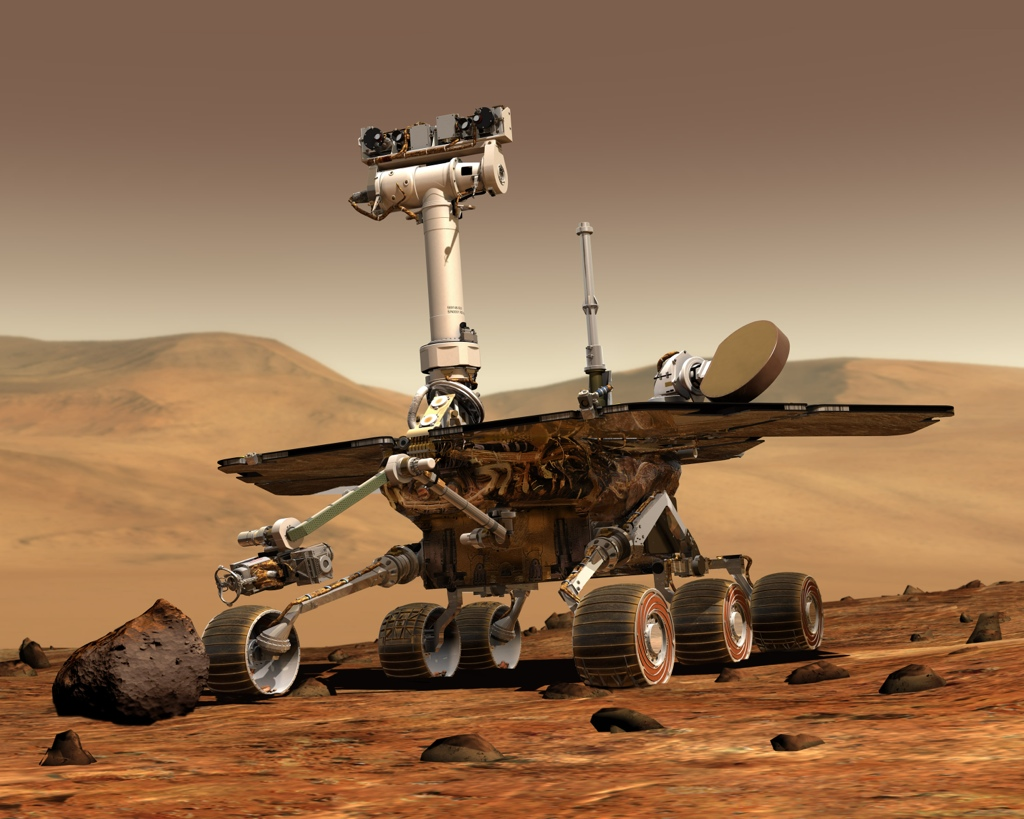
\includegraphics[width=0.7\linewidth]{bilder/nasa_rover}
		\caption{}
		\label{fig:nasarover}
	\end{figure}
	
	\cite{Kornmeier2011}
	\blindtext[4]
	\subsection{Unterabschnitt}
	
	\blindtext[5]
	
	\subsubsection{Unter-Unterabschnitt}
	
	\blindtext[5]
	
	\paragraph{Eine weitere Überschrift}
	
	\begin{figure*}
		\centering
		
\includegraphics[width=0.7\linewidth]{bilder/nature}
		\caption{}
		\label{fig:nature}
	\end{figure*}
	
	
	\subparagraph{Noch eine kleinere Überschrift}
	
	\subsection{Weiterer Unterabschnitt}
	
	\begin{align*} 
		2x - 5y &=  8 \\ 
		3x + 9y &=  -12
	\end{align*}
	
	\subsubsection{Unter-Unterabschnitt}
	
	
	\begin{enumerate}
		\item Eintrag 1
		\item Eintrag 2
		\item Eintrag 3
	\end{enumerate}
	
	\section{Tabellen}
	
	Tabellen werden normalerweise ohne vertikale Striche gesetzt, sondern die Spalten werden durch einen entsprechenden Abstand voneinander getrennt.\footnote{Siehe \cite[S. 89]{Willberg2021}.} Zum Einsatz kommen ausschließlich horizontale Linien (siehe \autoref{Kap2:Kopplungsformen}).
	
	\begin{table}[ht]
		\caption{Ebenen der Kopplung und Beispiele für enge und lose Kopplung}
		\label{Kap2:Kopplungsformen}
		\renewcommand{\arraystretch}{1.2}
		\centering
		\resizebox{\linewidth}{!}{  
			\begin{tabular}{l l l}
				\toprule
				\textbf{Form der Kopplung} & \textbf{enge Kopplung} & \textbf{lose Kopplung}\\
				\midrule
				Physikalische Verbindung	&	Punkt-zu-Punkt	& 	über Vermittler\\
				Kommunikationsstil	&	synchron		&	asynchron\\
				Datenmodell	&	komplexe gemeinsame Typen	&	nur einfache gemeinsame Typen\\
				Bindung	&	statisch		&	dynamisch\\
				\bottomrule
			\end{tabular}
		}
	\end{table}
	
	
	\begin{table*}[ht]
		\caption{Ebenen der Kopplung und Beispiele für enge und lose Kopplung}
		\label{Kap2:KopplungsformenA}
		\renewcommand{\arraystretch}{1.2}
		\centering
			\begin{tabular}{l l l}
				\toprule
				\textbf{Form der Kopplung} & \textbf{enge Kopplung} & \textbf{lose Kopplung}\\
				\midrule
				Physikalische Verbindung	&	Punkt-zu-Punkt	& 	über Vermittler\\
				Kommunikationsstil	&	synchron		&	asynchron\\
				Datenmodell	&	komplexe gemeinsame Typen	&	nur einfache gemeinsame Typen\\
				Bindung	&	statisch		&	dynamisch\\
				\bottomrule
			\end{tabular}
	\end{table*}
	
	\appendix
	
	\section{Der erste Anhang}
	
	\subsection{Mit einem Unteranschnitt}
	
	


\end{document}